\chapter{Experimente}\label{chap:experiments}

Nach der Beschreibung des Konzept und Verlauf des Python-Skripts geht dieses Kapitel auf die wichtigsten Trainingsdurchläufe ein und diskutiert die Ergebnisse. 
\\\\
Es wurden iterativ Trainingprozeduren durchgeführt mit jeweils unterschiedlichen Konfiguration, wie um vorherigen Kapitel gezeigt, und miteinander verglichen. Die genauen Konfigurationen werden bei den einzelnen Experimenten angeführt. Die Experimente liefen auf einem Rechner mit NVIDIA TITAN Xp 12 GB VRAM Grafikkarte, Intel i7-7800X CPU und 32 GB RAM. Da diese Arbeit zeitlich begrenzt ist, wurden die Experimente auf max. 100 Epochen begrenzt, was die durchschnittliche Laufzeit auf etwa drei bis vier Stunden je Experiment bringt. Diese Beschränkung wirkt ebenfalls Overfitting entgegen, da nicht ausreichend Zeit hat, um sich auf den Trainingsdatensatz "`einzugewöhnen"'.
\\\\
Es wurden drei unterschiedliche Datensätze aus den Sentinelprodukten erzeugt. 
\begin{enumerate}
	\item Der originale unaugmentierte Datensatz enthält insgesamt jeweils zwölf Bilder und Masken\footnote{Trainingsanteil: 7, Validationsanteil: 2, Testanteil: 3} und dient als Basis für das Ausgangsexperiment. 
	\item Der augmentierte Datansatz (s. Kapitel \ref{sec:augmentation}) enthält 1291 Dateien und Masken\footnote{Trainingsanteil: 825, Validationsanteil: 207, Testanteil: 259}. Nachdem die zufällige Ausschnitte produziert wurden, kam es vor, dass einige Masken keinen \textit{RoI}-Anteil enthielten. Diese Masken und auch die zugehörigen Bilddateien wurden verworfen und weicht deswegen von der eigentlichen Größe von 1296 Elementen\footnote{Die zwölf ursprünglichen Dateien multipliziert mit dem Data Augmentation-Faktor von 108.} ab.
	\item In einem dritten Datensatz wurden Ausschnitte benutzt, deren Bildgrenzen sich an den äußersten Punkten der Masken befinden (s. Abb. \ref{fig:example-overfitting}). Dieser Datensatz wurde ausschließlich mittels Rotationen erweitert und enthält 144 Elemente\footnote{Trainingsanteil: 92, Validationsanteil: 23, Testanteil: 29}. 
\end{enumerate}
\noindent

\section{Training mit Rohdaten}\label{sub:sub:sec:experiment-1}

\begin{lstlisting}[language=python,caption={Konfiguration für Experimente 1},captionpos=b]
class CropDiseaseConfig(Config):
    BACKBONE = "resnet50"
    IMAGE_MAX_DIM = 128
    IMAGE_MIN_DIM = 128
    IMAGE_RESIZE_MODE = "square"
    IMAGES_PER_GPU = 4
    LEARNING_RATE = 0.001
    NUM_CLASSES = 1 + 1
    RPN_ANCHOR_SCALES = (8, 16, 32, 64, 128)
    STEPS_PER_EPOCH = 23
    USE_MINI_MASK = False
\end{lstlisting}
\noindent
Zuerst wurden ein Modell auf Datensatz 1 und alle Schichten des Modells wurden trainiert. Diese Experimente sollen zeigen, wie ein zu kleiner Datensatz sich auswirken kann.

\begin{figure}[ht]
	\centering
    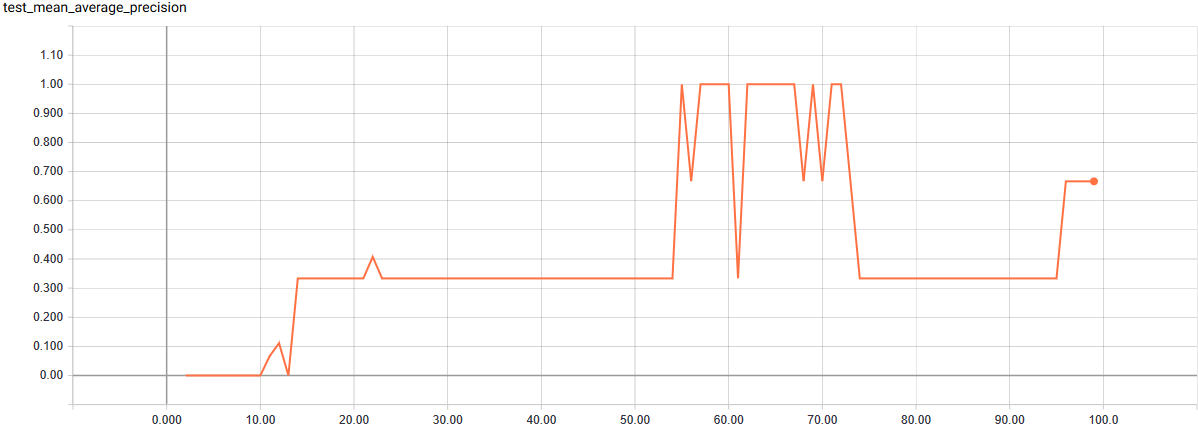
\includegraphics[width=.7\textwidth]{pics/map-1.PNG}
    \caption{\textit{mAP}-Graph von Experiment 1, X-Achse: Epochennummer, Y-Achse: \textit{mAP}-Werte}
    \label{fig:map-1}
\end{figure}
\begin{figure}[ht]
	\centering
    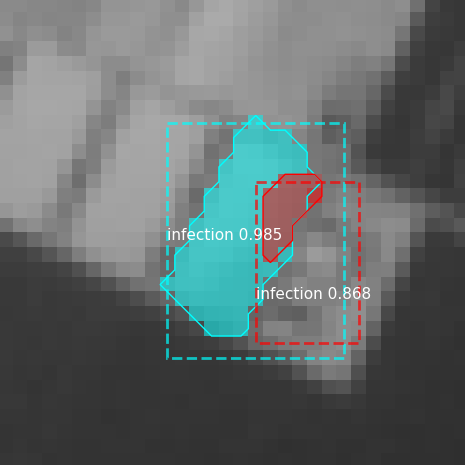
\includegraphics[height=3.5cm]{pics/pred-1-1.png}
    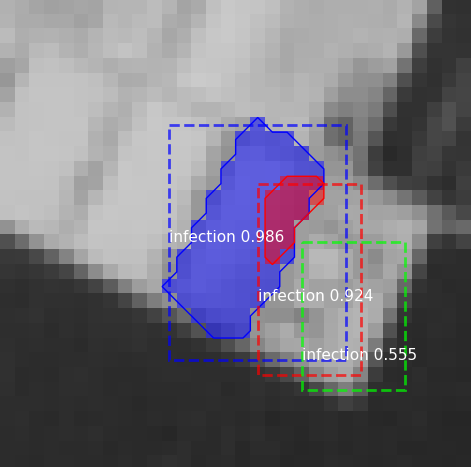
\includegraphics[height=3.5cm]{pics/pred-1-2.png}
    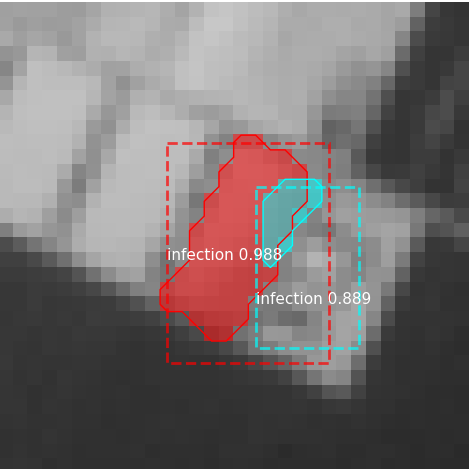
\includegraphics[height=3.5cm]{pics/pred-1-3.png}
    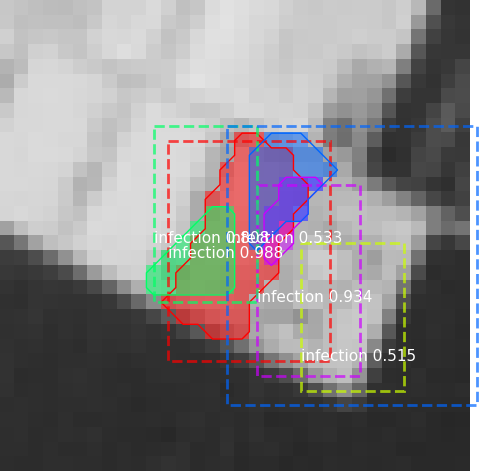
\includegraphics[height=3.5cm]{pics/pred-1-4.png}
    \caption[Beispielvorhersagen Experiment 1]{Beispielvorhersagen anhand der Gewichte von Epoche 55}
    \label{fig:pred-1}
\end{figure}
\noindent
Man sieht, dass das Modell während des Trainings unterdurchschnittliche Ergebnisse erzielt, was wenig überraschend ist, da der Datensatz sehr klein ist. Da nach jeder Epoche die Gewichte zwischengespeichert werden, können diese einzeln geladen werden. So wurde für eine Detektion ein Modell mit den Gewichten der 55. Epoche initialisiert, da sich hier der \textit{mAP}-Wert auf dem Maximalwert befindet. Die Bilder in Abb. \ref{fig:pred-1} entstammen einem fremden Datensatz, ähneln aber in den Grundcharakteristika dem eigentlichen Datensatz 1. Zum Beispiel ist das Zielfeld ähnlich ausgerichtet und zentriert. Man sieht, dass sich die berechneten Masken relativ genau auf das Zielfeld eingrenzen. Jedoch sind die erzeugten Bounding-Boxen und passen nicht zu den entsprechenden Masken, falls eine Maske erkannt wurde. Auch wurden mehrere Objektinstanzen erkannt, wobei eine einzige Instanz detektiert werden sollte. Werden die Bilder in Abb. \ref{fig:pred-1} nun vertikal gespiegelt und in das Netzwerk gegeben, erzeugt das Modell keine Masken, obwohl lediglich die Ausrichtung verändert wurde. Das ist ein Hinweis auf Overfitting, da das neuronale Netz minimale Änderungen nicht mehr erkennt.

\section{Datensatzerweiterung durch Rotation}\label{sub:sub:sec:experiment-2}

\begin{lstlisting}[language=python,caption={Konfiguration für Experiment 2},captionpos=b]
class CropDiseaseConfig(Config):
    BACKBONE = "resnet50"
    IMAGE_MAX_DIM = 128
    IMAGE_MIN_DIM = 128
    IMAGE_RESIZE_MODE = "square"
    IMAGES_PER_GPU = 4
    LEARNING_RATE = 0.001
    NUM_CLASSES = 1 + 1
    RPN_ANCHOR_SCALES = (8, 16, 32, 64, 128)
    STEPS_PER_EPOCH = 206
    USE_MINI_MASK = False
\end{lstlisting}
\noindent
Bei diesem Experiment wurde ein Modell Datensatz 3 und alle Schichten des Modells trainiert. Die Konfiguration bleibt unverändert, jedoch ist hier der augementierte Datensatz vergleichweise größer.

\begin{figure}[ht]
	\centering
    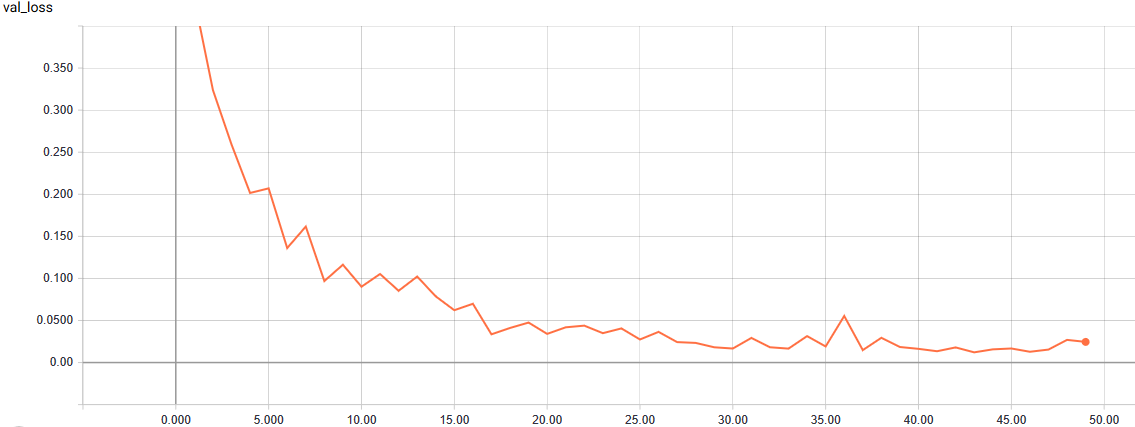
\includegraphics[width=.7\textwidth]{pics/val-loss-2.PNG}
    \caption{\textit{loss}-Graph von Experiment 2, X-Achse: Epochennummer, Y-Achse: \textit{loss}-Werte}
    \label{fig:val-loss-2}
\end{figure}

\begin{figure}[ht]
	\centering
    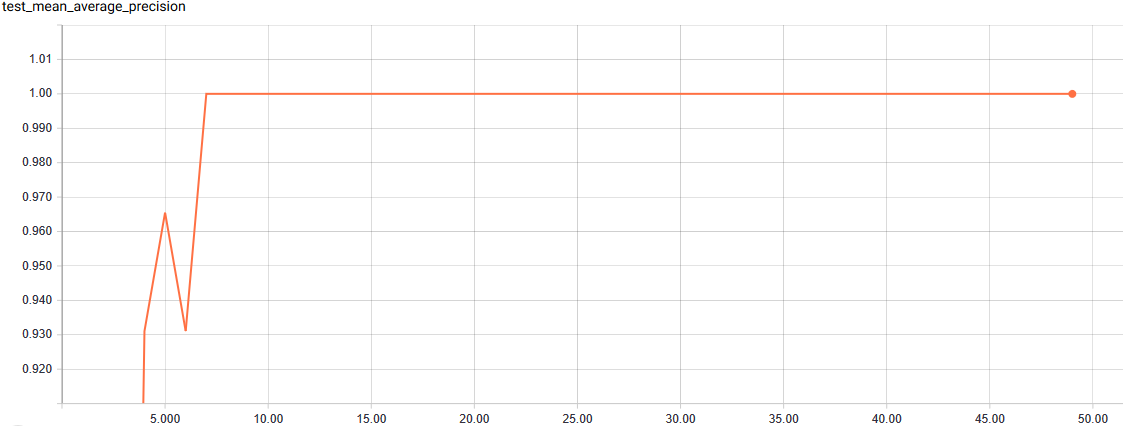
\includegraphics[width=.7\textwidth]{pics/map-2.PNG}
    \caption{\textit{mAP}-Graph von Experiment 2, X-Achse: Epochennummer, Y-Achse: \textit{mAP}-Werte}
    \label{fig:map-2}
\end{figure}

\begin{figure}[ht]
  \centering
  \begin{minipage}[c]{.3\textwidth}
  \centering
  
\includegraphics[height=2cm]{pics/roi-2-1.png}
  \\ \vspace{.25cm}
  
\includegraphics[height=3cm]{pics/roi-2-2.png}
  \\ \vspace{.25cm}
  
\includegraphics[height=3cm]{pics/roi-2-3.png}
  \\ \vspace{.25cm}
  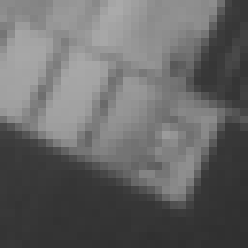
\includegraphics[height=3cm]{pics/roi-2-4.png}
  \end{minipage}
  \begin{minipage}[c]{.3\textwidth}
  \centering
  
\includegraphics[height=2cm]{pics/mask-2-1.png}
  \\ \vspace{.25cm}
  
\includegraphics[height=3cm]{pics/mask-2-2.png}
  \\ \vspace{.25cm}
  
\includegraphics[height=3cm]{pics/mask-2-3.png}
  \\ \vspace{.25cm}
  
\includegraphics[height=3cm]{pics/mask-2-4.png}
  \end{minipage}
  \begin{minipage}[c]{.3\textwidth}
  \centering
  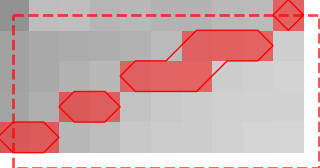
\includegraphics[height=2cm]{pics/pred-2-1.png}
  \\ \vspace{.25cm}
  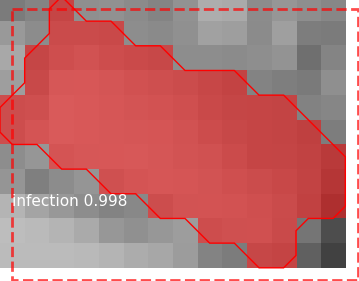
\includegraphics[height=3cm]{pics/pred-2-2.png}
  \\ \vspace{.25cm}
  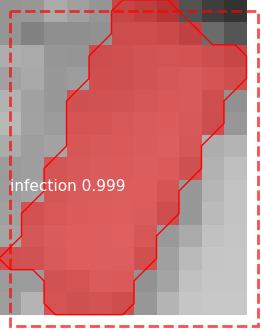
\includegraphics[height=3cm]{pics/pred-2-3.png}
  \\ \vspace{.25cm}
  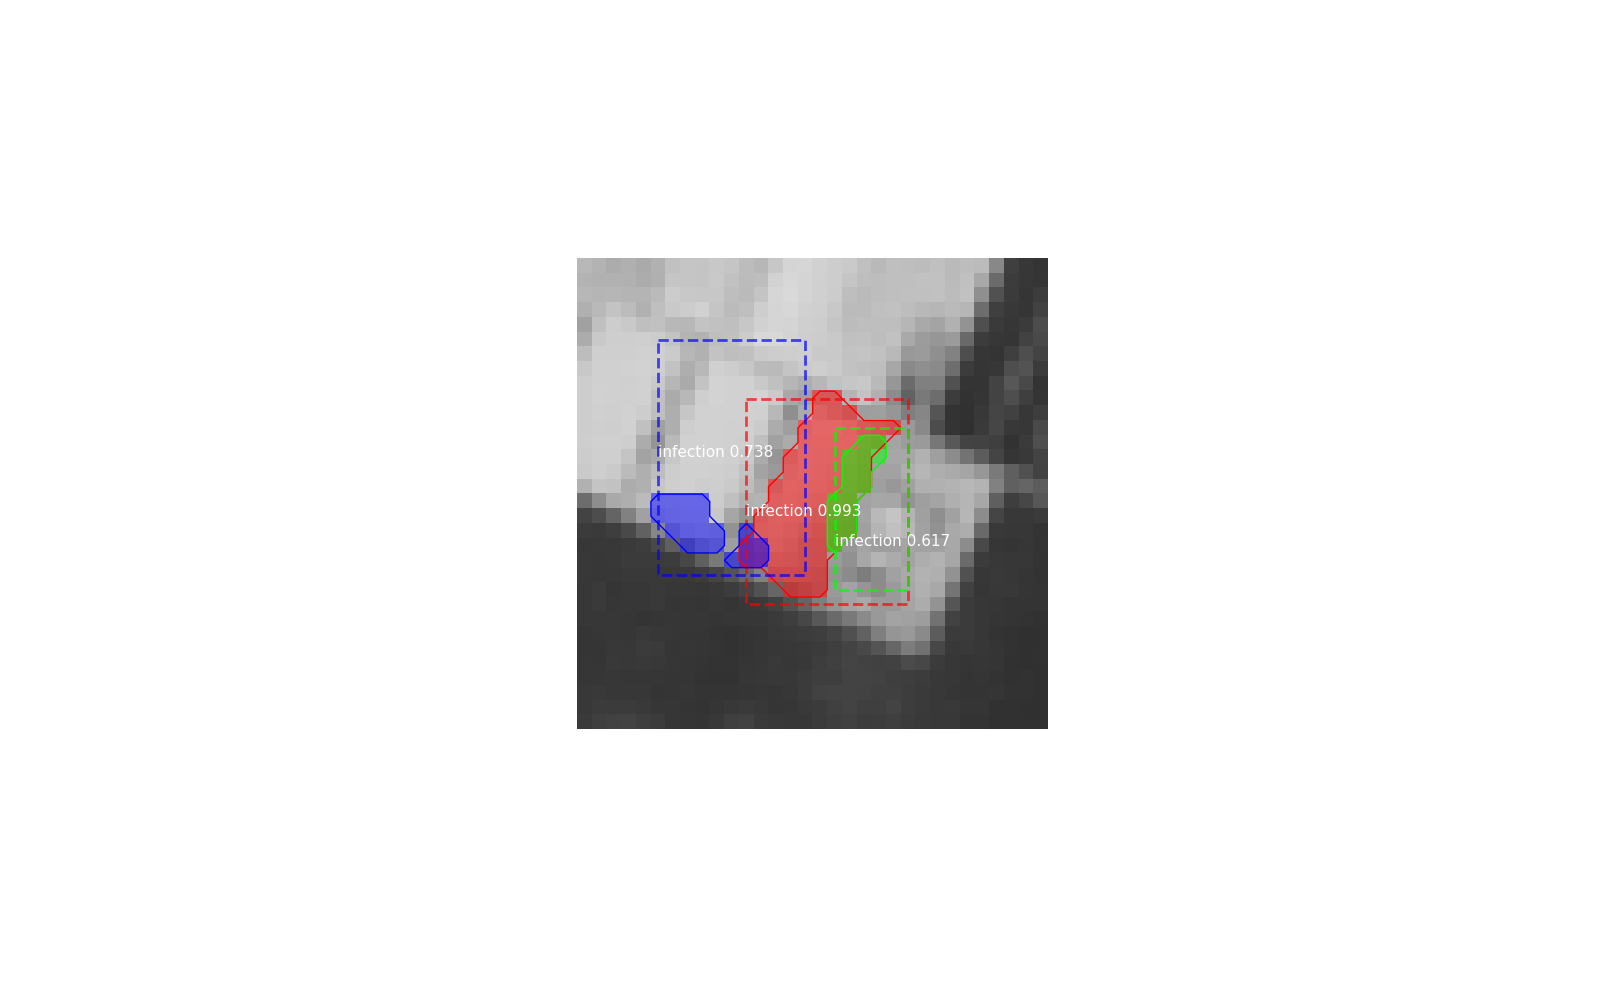
\includegraphics[height=3cm]{pics/pred-2-4.png}
  \end{minipage}

  \caption[Beispielvorhersagen Experiment 2]{Beispielvorhersagen anhand der Gewichte von Epoche 37, links: Ausgangsbild, mitte: Maske, rechts: Detektion}
  \label{fig:pred-2}
\end{figure}
\noindent
Die \textit{mAP}-Kurve konvergiert ab Epoche 7 gegen $1$ und verweilt dort für den Rest des Trainings. Dagegen sinken die $loss$-Werte weiterhin und nähern sich ab Epoche 37 $0$ an. Daher wurde die Gewichte dieser Epoche näher untersucht. Abb. \ref{fig:pred-2} zeigt, dass das Modell resistenter gegenüber Rotationen ist. Nichtsdestotrotz reagiert das Modell empfindlich auf Veränderungen wie zum Beispiel ein größerer Ausschnitt oder Translationen (s. unterste Reihe in Abb. \ref{fig:pred-2}). Daraus ergibt sich, dass das Modell nicht allgemein einsetzbar ist und die Daten durch weitere Augmentationen randomisiert werden müssen.
\newpage
\section{Data Augmention und Regularization}\label{sec:experiment-3}

\begin{lstlisting}[language=python,caption={Konfiguration für Experiment 3},captionpos=b,label=lst:experiment-3]
class CropDiseaseConfig(Config):
    BACKBONE = "resnet50"
    IMAGE_MAX_DIM = 128
    IMAGE_MIN_DIM = 128
    IMAGE_RESIZE_MODE = "square"
    IMAGES_PER_GPU = 4
    LEARNING_RATE = 0.001
    NUM_CLASSES = 1 + 1
    RPN_ANCHOR_SCALES = (8, 16, 32, 64, 128)
    STEPS_PER_EPOCH = 3
    USE_MINI_MASK = False
    WEIGHT_DECAY = 0.0001 # Orange, Dunkelblau, Rot
    WEIGHT_DECAY = 0.001 # Pink
    WEIGHT_DECAY = 0.01 # Hellblau
\end{lstlisting}
\noindent
Diese Sektion vergleicht mehrere Traingsläufe direkt miteinander. Zur simpleren Kommunikation werden die einzelnen Durchläufe mit den Farben betitelt, wie sie in den Graphen \ref{fig:val-loss-3} und \ref{fig:map-3} (Orange, Rot, Pink, Hell- und Dunkelblau) repräsentiert sind. Die verschiedenen \texttt{WEIGHT\_DECAY}-Werte in Listing \ref{lst:experiment-3} sind in den entsprechenden Modellkonfigurationen zu verwenden, wie sie in den Kommentaren benannt sind, wobei der Wert für die orangene, rote und dunkelblaue Konfigurationen implizit in der Basisklasse \texttt{Config} definiert ist. Die pinke und hellblaue Konfiguration soll den Einfluss von L2 Regularization zeigen. Alle Modelle bis auf das orangene wurden auf Grundlage von Datensatz 2 trainiert. Aus Gründen, die später erklärt werden, wurde für das orangene Modell ein Datensatz kreiert, das sich auf die kleine Zone innerhalb des Feldes mit der stärkeren Infektionskonzentration beschränkt. Der \textit{head} des dunkelblauen Netzwerk wurde trainiert, während alle Schichten der restlichen Modelle trainiert wurden.

\begin{figure}[ht]
	\centering
    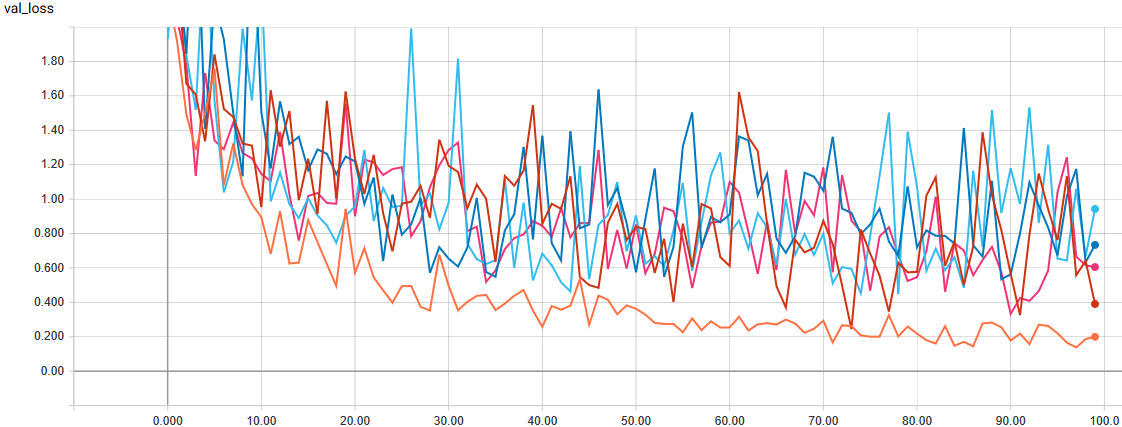
\includegraphics[width=.7\textwidth]{pics/val-loss-3.PNG}
    \caption{\textit{loss}-Graph von Experiment 2, X-Achse: Epochennummer, Y-Achse: \textit{loss}-Werte}
    \label{fig:val-loss-3}
\end{figure}

\begin{figure}[ht]
	\centering
    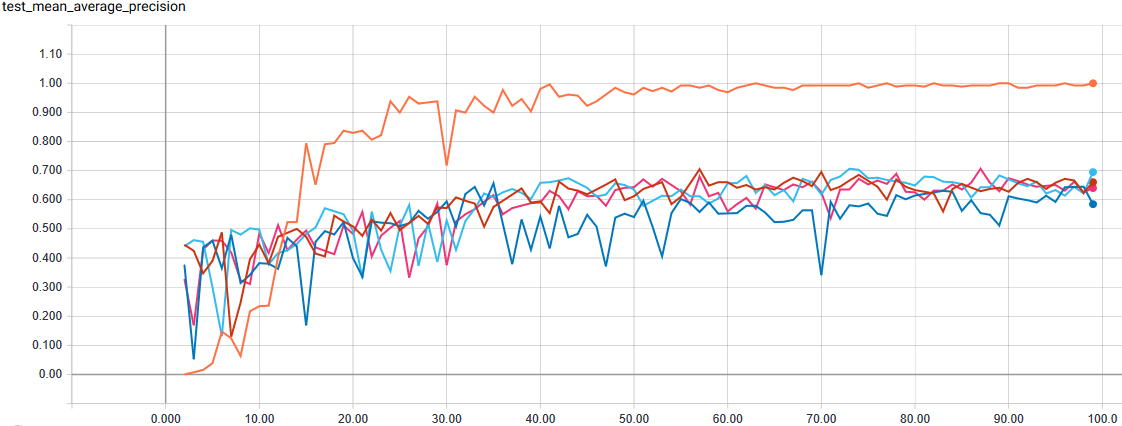
\includegraphics[width=.7\textwidth]{pics/map-3.PNG}
    \caption{\textit{mAP}-Graph von Experiment 2, X-Achse: Epochennummer, Y-Achse: \textit{mAP}-Werte}
    \label{fig:map-3}
\end{figure}

\begin{figure}[H]
  \centering
  \begin{minipage}[c]{.3\textwidth}
  \centering
  
\includegraphics[height=3cm]{pics/roi-3-2.png}
  \\ \vspace{.25cm}
  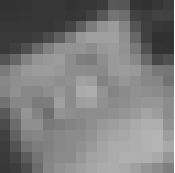
\includegraphics[height=3cm]{pics/roi-3-3.png}
  \\ \vspace{.25cm}
  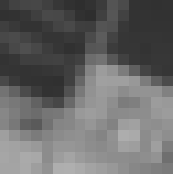
\includegraphics[height=3cm]{pics/roi-3-4.png}
  \\ \vspace{.25cm}
  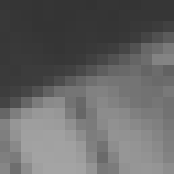
\includegraphics[height=3cm]{pics/roi-3-5.png}
  \\ \vspace{.25cm}
  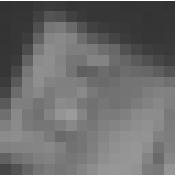
\includegraphics[height=3cm]{pics/roi-3-1.png}
  \end{minipage}
  \begin{minipage}[c]{.3\textwidth}
  \centering
  
\includegraphics[height=3cm]{pics/mask-3-2.png}
  \\ \vspace{.25cm}
  
\includegraphics[height=3cm]{pics/mask-3-3.png}
  \\ \vspace{.25cm}
  
\includegraphics[height=3cm]{pics/mask-3-4.png}
  \\ \vspace{.25cm}
  
\includegraphics[height=3cm]{pics/mask-3-5.png}
  \\ \vspace{.25cm}
  
\includegraphics[height=3cm]{pics/mask-3-1.png}
  \end{minipage}
  \begin{minipage}[c]{.3\textwidth}
  \centering
  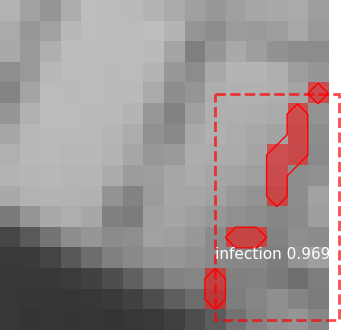
\includegraphics[height=3cm]{pics/pred-3-2.png}
  \\ \vspace{.25cm}
  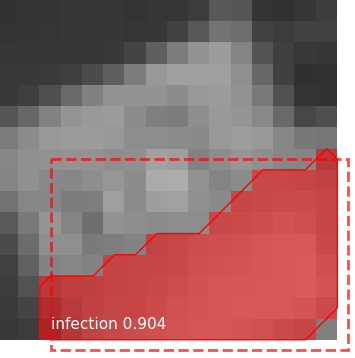
\includegraphics[height=3cm]{pics/pred-3-3.png}
  \\ \vspace{.25cm}
  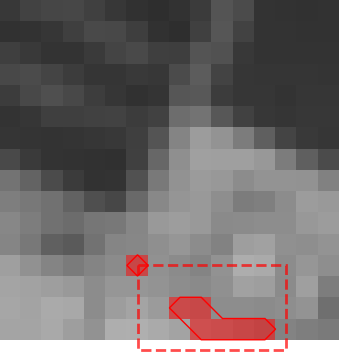
\includegraphics[height=3cm]{pics/pred-3-4.png}
  \\ \vspace{.25cm}
  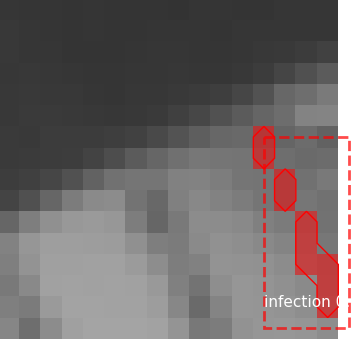
\includegraphics[height=3cm]{pics/pred-3-5.png}
  \\ \vspace{.25cm}
  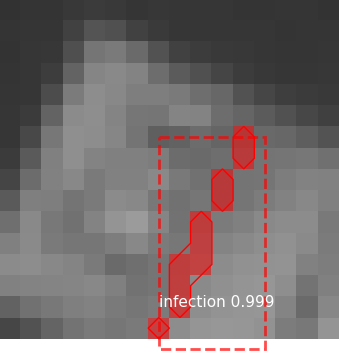
\includegraphics[height=3cm]{pics/pred-3-1.png}
  \end{minipage}

  \caption[Beispielvorhersagen Experiment 2]{Beispielvorhersagen verschiedener Modelle, v.l.n.r.: Ausgangsbild, Masken, Vorhersage, v.o.n.u.: Vorhersagen von dunkelblau, rot, hellblau, pink, orange}
  \label{fig:pred-3}
\end{figure}
\noindent
Für auf Datensatz 3 trainierten Modelle (jeweils Epoche 100) zeichnen sich in  Abb. \ref{fig:val-loss-3} starke Schwankungen ab und kein Modell überschreitet $mAP>0.7$. Die Vorhersagen in den oberen vier Reihen in Abb. \ref{fig:pred-3} stimmen zum großen Teil mit den Masken überein. Weitere hier nicht aufgeführte Vorhersagen zeigen ähnliche Ergebnisse. Es kommt vor, dass die kleine Zielregion vorhergesagt wird, obwohl die entsprechende binäre Maske die große \textit{RoI} repräsentiert, so ähnlich wie es in der unteren Reihe zu sehen ist. Dieses Verhalten würde die schlechten \textit{mAP}-Kurven und die Schwankungen erklären. Da die Detektion nicht mit dem erwarteten Ergebnis übereinstimmt und daher der berechnete Fehler größer ist, obwohl die Detektion eigentlich korrekt ist, da sich beide genutzten \textit{RoIs} geografisch schneiden. Durch den größeren Fehler ist die Korrektur der Gewichte entsprechend größer. Um die Annahme zu bekräftigen, wurde ein Modell (orange) auf dem speziellen Datensatz trainiert. Im Vergleich zu den anderen Kurven konvergiert die orangene \textit{loss}-Kurve gegen $0$ bzw. die orangene \textit{mAP}-Kurve gegen $1$. Wäre mehrere unterschiedliche \textit{RoIs} vorhanden, die sich nicht schneiden, würde der Einfluss sich nicht bemerkbar machen. Was hier jedoch nicht der Fall ist, da beide \textit{RoIs} jeweils etwa die Hälfte des Datensatzes ausmachen.
\\\\
Es ist zu sehen, dass die \textit{Ridge Regression} (hellblau und pink) keinen merkbaren Einfluss auf das Training haben, weil einen ähnlichen Verlauf wie die dunkelblaue und rote Kurven haben. Im Gegensatz dazu zeigt die \textit{Data Augmentation} positive Ergebnisse (s. Abb. \ref{fig:pred-3}) und alle Modelle sind deutlich robuster gegenüber manipulierten Bildern. Jedoch schlagen die Detektionen bei größeren Ausschnitten fehl oder geben sinnlose Resultate zurück. Weiterhin sei erwähnt, dass das Modell, dessen \textit{head} trainiert wurde, von allen hier erwähnten Modellen am schlechtesten abschneidet und es zumindest nicht hilfreich ist, nur die oberen Schichten zu trainieren.